\documentclass{beamer}

% === AUTOR === (((
\author{\textit{Por Erick I. Rodríguez Juárez.}}
% )))

% === PAQUETES === (((
% \usepackage{makeidx}
% \usepackage{xltxtra}
\usepackage{amsfonts}
\usepackage{amsmath}
\usepackage{amssymb}
% \usepackage{fullpage}
\usepackage{tikz}
\usetikzlibrary{arrows.meta}
\usepackage{graphicx}
% )))

% === TIPOGRAFÍA === (((
% \setmainfont[
  % BoldFont       = bodonibi,
	% ItalicFont     = Century modern italic2.ttf,
	% BoldItalicFont = bodonibi,
	% SmallCapsFont  = lmromancaps10-regular.otf
% ]{Century_modern.ttf}
% )))

% === COMANDOS === (((
% \newcommand{\dis}{\displaystyle}
% \newcommand{\qed}{\hspace{0.5cm}\rule{0.16cm}{0.4cm}}
% \newcommand{\operator}[1]{\mathop{\vphantom{\sum}\mathchoice
% {\vcenter{\hbox{\huge $#1$}}}
% {\vcenter{\hbox{\Large $#1$}}}{#1}{#1}}\displaylimits}
% \newcommand{\suma}{\operator{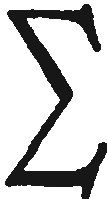
\includegraphics[scale=0.09]{FOTOS/Sigma.png}}}
% \setlength{\parindent}{0mm}
% )))

% === ITALICA EN ENTORNO MATEMÁTICO === (((
% \DeclareSymbolFont{italics}{\encodingdefault}{\rmdefault}{m}{it}
% \DeclareSymbolFontAlphabet{\mathit}{italics}
% \ExplSyntaxOn
% \int_step_inline:nnnn { `A } { 1 } { `Z }
 % {  \exp_args:Nf \DeclareMathSymbol{\char_generate:nn{#1}{11}}{\mathalpha}{italics}{#1} }
% \int_step_inline:nnnn { `a } { 1 } { `z } {  \exp_args:Nf \DeclareMathSymbol{\char_generate:nn{#1}{11}}{\mathalpha}{italics}{#1}}
% \ExplSyntaxOff
% )))

\begin{document}

\frame{\titlepage}

\begin{frame}[t]
	\begin{block}{}
		El concepto de un movimiento armónico simple no es realista, a menos que la masa esté colgada en un vacío perfecto, ya que al menos bará una fuerza de resistencia debida al medio que lo rodea.
		En mecánica, se considera que las fuerzas de amortiguamiento que actúan sobre un cuerpo son proporcionales a alguna potencia de la velocidad instantánea.
		En particular, supondremos que ésta fuerza es proporcional a la derivada de \(x\) con respecto al tiempo.
		\begin{minipage}{0.4\linewidth}
			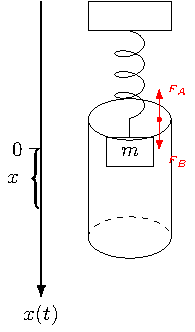
\includegraphics[width= 0.6 \linewidth]{IMAGENES/1/tikz.pdf}
		\end{minipage}\hspace{5mm}
		\begin{minipage}{0.5\linewidth}
			La fuerza total que se ejerce sobre la masa es:
			\[
				F_T = -kx- \beta x'.
			\]
			Por la \(2^{da}\) Ley de Newton \(F_T=ma=mx'\). \\[2mm]
			Por lo cual, se tiene
			\[
				mx'' = -kx - \beta x'.
			\]
		\end{minipage}
	\end{block}
\end{frame}

\begin{frame}[t]
	\begin{block}{}
		\[
			\begin{array}{rrcl}
				\iff & mx'' + \beta x' + kx & = & 0 \\[2mm]
				\iff & x'' + 2 \lambda x' + \omega ^2x & = & 0.\\
			\end{array}
		\]
		\[
			\underbrace{\hphantom{x'' + 2 \lambda x' + \omega ^2x = 0}}_\text{\color{red} E.D.O. de \(2^{do}\) Orden lineal homogénea coef. const.} 
		\]
		donde \(2 \lambda = \beta /m\), \(\omega ^2 = k/m\). \\[2mm]
		Esta E.D. está sujeta a la C.I. \(x(0) = x_0\), \(x' (0) = x_1\).
		Resolvemos este P.V.I., usando la ecuación característica:
		\[
			m^2+2 \lambda m + \omega ^2 =0.
		\]
		\[
			\begin{array}{rcl}
				m_{1,2} & = & \dfrac{-2 \lambda \pm \sqrt{(2 \lambda) ^2 - 4(\omega ^2)}}{2}\\[2mm]
				& = & - \lambda \pm \sqrt{\lambda ^2- \omega ^2} .
			\end{array}
		\]
		Se tienen \(3\) casos.
	\end{block}
\end{frame}

\begin{frame}[t]
	\begin{block}{}
		\begin{enumerate}
			\item \fbox{\(\lambda ^2- \omega ^2 >0\)} raíces reales y distintas negativas \(m_1,m_2\) 
				\[
					\begin{array}{c}
						x(t) = c_1e^{m_1t} + c_2e^{m_2t}. \\[2mm]
						\dis\lim_{t\rightarrow \infty} x(t) =0, \hspace{5mm} \mbox{la masa tiende al equilibrio resorte.}
					\end{array}
				\]
				\begin{minipage}{0.4\linewidth}
					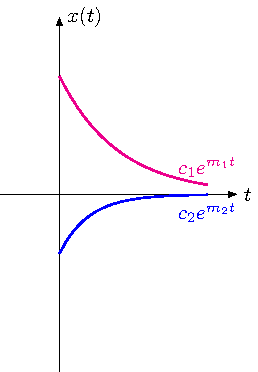
\includegraphics[width= 0.9 \linewidth]{IMAGENES/3/tikz.pdf}
				\end{minipage}\hspace{5mm}
				\begin{minipage}{0.5\linewidth}
					En este caso, se dice que el sistema está sobreamortiguado.
				\end{minipage}
		\end{enumerate}
	\end{block}
\end{frame}

\begin{frame}[t]
	\begin{block}{}
		\begin{enumerate}
			\setcounter{enumi}{1}
			\item \fbox{\(\lambda ^2-w^2=0\)} Se tienen dos raíces iguales negativas \(m_1=m_2 = -\lambda <0\),
				\[
					\begin{array}{rcl}
						x(t) & = & c_1e^{- \lambda x} c_2+c_3e^{- \lambda t}. \\[2mm]
						\dis\lim_{t\rightarrow 0} e^{- \lambda t} (c_1+c_2t) & \stackrel{L'Hoptial}{=}  & \dis\lim_{t\rightarrow a} \dfrac{c_2}{\lambda e^{\lambda t}} =0.
					\end{array}
				\]
				\begin{minipage}{0.5\linewidth}
					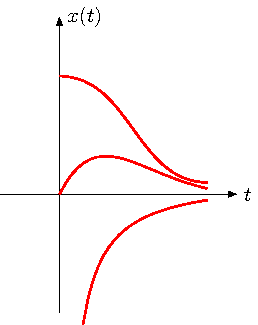
\includegraphics[width= 0.8 \linewidth]{IMAGENES/4/tikz.pdf}
				\end{minipage}
				\begin{minipage}{0.4\linewidth}
					Sistema críticamente amortiguado.
				\end{minipage}
		\end{enumerate}
	\end{block}
\end{frame}

\begin{frame}[t]
	\begin{block}{}
		\begin{enumerate}
			\setcounter{enumi}{2}
		\item \fbox{\(\lambda ^2- w^2 < 0\)} Se tienen \(2\) raíces complejas, \(m_{1,2} = - \lambda \pm i \sqrt{w^2- \lambda ^2}\).
			\[
				\alpha = - \lambda \hspace{1cm} \gamma = \sqrt{w^2-  \lambda ^2}.
			\]
				\color{red} \vspace{-5mm}
			\[
				\begin{array}{rcl}
					\color{black} x(t) & \color{black} = & \color{black} c_1e^{- \lambda t} \cos (\gamma t) +c_2e^{- \lambda t} \sin (\gamma t) \\ \hline
					\color{black} & \color{black} = & \color{black} e^{- \lambda t} \cdot A \sin (\gamma t+ \varphi)
				\end{array}
			\]
				\begin{figure}[hbtp!]
					\centering
					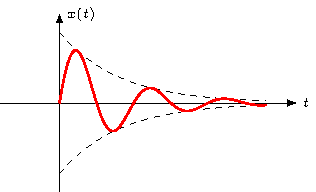
\includegraphics[width= 0.8 \linewidth]{IMAGENES/5/tikz.pdf}
				\end{figure}
		\end{enumerate}
	\end{block}
\end{frame}

\begin{frame}[t]
	\begin{alertblock}{Ejercicio.}
		Un contrapeso de \(8lb\) estira \(2ft\) a un resorte. Si una fuerza de amortiguamiento numéricamente igual a \(2x\,'\) actúa sobre el sistema, deduzca la ecuación del movimiento si el contrapeso se suelta de la posición de equilbrio con una velocidad hacia arriba de \(3ft/s\).
	\end{alertblock}
\end{frame}
\begin{frame}[t]
\end{frame}

\begin{frame}[t]
	\frametitle{Sistema Masa-Resorte.}
	\begin{block}{}
		Si tenemos en cuenta una fuerza externa \(F\), la cual se aplica sobre la masa oscilatoria en un resorte se obtiene lo siguiente:\\[3mm]
		\begin{minipage}{0.3\linewidth}
			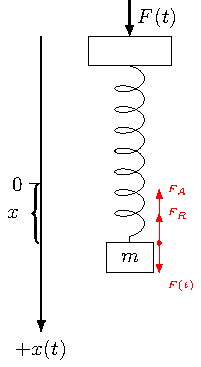
\includegraphics[width= \linewidth]{IMAGENES/6/tikz.pdf}
		\end{minipage}\hspace{5mm}
		\begin{minipage}{0.6\linewidth}
			\(F(t) \;:\;\) fuerza externa sobre la masa, que causa un movimiento vertical del soporte del resorte.
			\[
				F_t = -kx -bx\,' +F(t).
			\]
			Por la \(2^{da}\) Ley de Newton,
			\[
				F_T = ma  =mx\,''.
			\]
			\(\therefore\) La E.D. que modela el sistema masa--resorte con fuerza externa es:
		\begin{center}
			\color{red} \underline{\(\color{black} mx\,'' + \beta x\,' +kx = F(t)\)}
		\end{center}
		\end{minipage}
	\end{block}
\end{frame}

\begin{frame}[t]
	\begin{block}{}
		Diremos que la ecuación diferencial representa un \textbf{fenómeno de vibraciones libres} si la fueza externa es nula. En caso contrario, diremos que se trata de un \textbf{modelo de vibraciones forzadas}.
	\end{block}
	\begin{block}{Vibraciones forazadas sin amortiguamiento \((\beta =0)\).}
		Cuando la fuerza es periódica (por ejemplo, \(F_0 \cos wt\)), y no  hay amortiguamiento \(\beta =0\), entonces la E.D. se reduce:
		\[
			x\,'' + w_0^2x = F_0 \cos wt.
		\]
		Se tienen dos casos:
		\begin{enumerate}
			\item Si \(w_0= \sqrt{k/m} \ne w\), entonces la solución es de la forma
				\[
					x(t) = c_1 \cos w_0t + c_2 \sin w_0t + \dfrac{F_0}{m(w_0^2- w^2)} \cos wt.
				\]
		\end{enumerate}
	\end{block}
\end{frame}

\begin{frame}[t]
	\begin{block}{}
		\color{red}{Pulsasiones:} \vspace{-5mm}
		\begin{figure}[hbtp!]
			\centering
			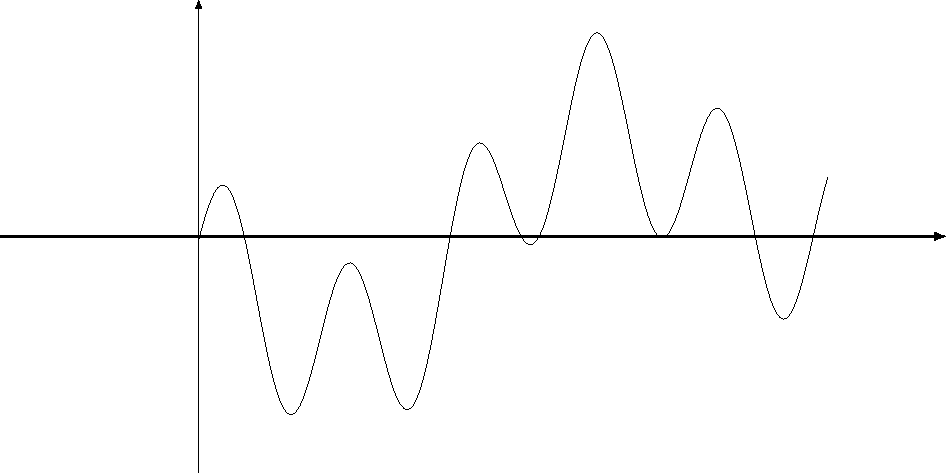
\includegraphics[width= 0.5 \linewidth]{IMAGENES/7/tikz.pdf}
		\end{figure}
		\begin{enumerate}
			\setcounter{enumi}{1}
			\item Si \(w=w_0\), la frecuencia de la función de la fuerza externa es igual a la frecuencia natural del sistema.
		\end{enumerate}
		\begin{figure}[hbtp!]
			\centering
			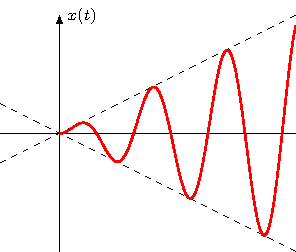
\includegraphics[width= 0.4 \linewidth]{IMAGENES/8/tikz.pdf}
		\end{figure}
	\end{block}
\end{frame}

\begin{frame}[t]
	\begin{block}{}
		La resonancia puede causar serias dificultades en el diseño de estructuras en donde puede producir inestabilidades y que pueden provocar la falla de las mismas. \\[2mm]
		Suponiendo que la fuerza es \(F_0 \cos wt\), la solución de la E.D. es de la forma:
		\[
			x(t) = \color{red} \underbrace{\color{black} c_1e^{r_1t} + c_2e^{r_2 t}} _{x_c(t)} \color{black}{+} \color{red} \underbrace{\color{black} R \cos (wt- \varphi)} _{x_p(t)}.
		\]
		Donde \(r_1\) y \(r_2\) satisfacen la ecuación característica asociada con la ecuación homogénea y en cualquier caso \(x_c(t) \longrightarrow 0\) cuando \(t \longrightarrow \infty\). \\[2mm]
		Por lo que se le conoce como \textbf{solución transitoria}. A \(x_p(t )\) que representa la oscilacij́on estable con la misma frecuencia que la fuerza externa se le llama \textbf{solución de estado estable} o \textbf{respuesta forzada}. 
	\end{block}
\end{frame}

\begin{frame}[t]
	\begin{block}{}
		\begin{figure}[hbtp!]
			\centering
			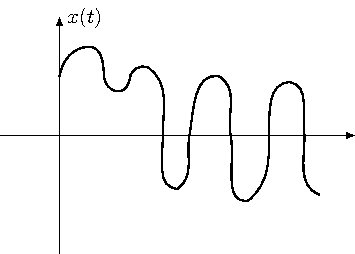
\includegraphics[width= 0.7 \linewidth]{IMAGENES/9/tikz.pdf}
		\end{figure}
	\end{block}
\end{frame}

\end{document}
